% THIS IS SIGPROC-SP.TEX - VERSION 3.1
% WORKS WITH V3.2SP OF ACM_PROC_ARTICLE-SP.CLS
% APRIL 2009
%
% It is an example file showing how to use the 'acm_proc_article-sp.cls' V3.2SP
% LaTeX2e document class file for Conference Proceedings submissions.
% ----------------------------------------------------------------------------------------------------------------
% This .tex file (and associated .cls V3.2SP) *DOES NOT* produce:
%       1) The Permission Statement
%       2) The Conference (location) Info information
%       3) The Copyright Line with ACM data
%       4) Page numbering
% ---------------------------------------------------------------------------------------------------------------
% It is an example which *does* use the .bib file (from which the .bbl file
% is produced).
% REMEMBER HOWEVER: After having produced the .bbl file,
% and prior to final submission,
% you need to 'insert'  your .bbl file into your source .tex file so as to provide
% ONE 'self-contained' source file.
%
% Questions regarding SIGS should be sent to
% Adrienne Griscti ---> griscti@acm.org
%
% Questions/suggestions regarding the guidelines, .tex and .cls files, etc. to
% Gerald Murray ---> murray@hq.acm.org
%
% For tracking purposes - this is V3.1SP - APRIL 2009

\documentclass{acm_proc_article-sp}
\usepackage{filecontents}

\begin{document}
\title{Latent Dirichlet Allocation as a Twitter Hashtag Recommender System
	\titlenote{There are no legal restrictions! Break all the rules! We don't own this, and wouldn't even dare claim it if our lives depended on it. Plagiarize to your heart's desire, but maybe hook us up with a job interview if you think we had some good ideas in here.}}



\numberofauthors{2} 
\author{
\alignauthor
Brian Gillespie\\
       \affaddr{Northeastern University}\\
       \affaddr{Seattle, WA}\\
       \email{bng1290@gmail.com}
\alignauthor
Shailly Saxena\\
       \affaddr{Northeastern University}\\
       \affaddr{Seattle, WA}\\
       \email{saxena.sha@husky.neu.edu}
}

\date{26 March 2016}



\maketitle
\begin{abstract}
\hspace*{5mm}In this paper, we investigate an unsupervised approach to hashtag recommendation, to aid in the classification of tweets. Two corpora were generated from a sample of tweets collected from September 2009 to January 2010. The first corpus was composed simply of individual tweets, and the second corpus was made by aggregating tweets by UserID into what is referred to as the USER PROFILE model. Latent Dirichlet Allocation(LDA) was used to generate topic distributions for each corpus, and then Collapsed Gibbs Sampling was used to generate topic distributions for new test tweets. By sampling a topic from each test tweet, and then sampling one of the top terms from that topic, a set of words can be selected as recommended hashtags. This recommendation process was applied to several example tweets, and the relevancy of the suggested hashtags were evaluated by human observers. The results of this would be briefly mentioned here if there were any.
\end{abstract}

\keywords{Twitter, LDA, topic modeling, NLP, social media} 

\section{Introduction}
\hspace*{5mm}Twitter is an amazing source of text data, both in content and quantity. With over 305 million monthly active users across the globe, there are a wide variety of subjects being discussed. Cataloging this data, and finding ways to make it more search-able is very desirable, as this data can be an effective resource for business knowledge and studying social trends. Hash-tags appears as the natural categorization index for tweets, however since only 8\% of tweets contain a hashtags, they cannot be used as a direct categorization for all tweets. Compounding this issue, there are no prescribed hashtags; any sequence of characters can be a hashtag as long as it has a \# in front of it. A hashtag recommendation system can be implemented to encourage users to utilize more hashtags, and to provide a more consolidated hashtag base for tweet categorization. But in order to avoid prescribing hashtags, and thus limiting the free expression of Twitter users, it is more reasonable to generate the suggested hashtags from the content of Twitter itself. This has the added gain of providing an adaptable system that can develop alongside the vocabulary and interests of the Twitter user base.

\section{Related Work}
\hspace*{5mm}There has been much research in the structure and dynamics of microblogging networks, and many insights have been gained by looking into how users interact with one another and with the world. Attempts to glean detailed information from the actual contents of the networks however, has met with limited success. Recent developments in topic-modeling approaches to Twitter data such as Hong and Davison\cite{hong2010empirical} and Zhao, Wayne Xin, et al.\cite{zhao2011comparing} have further refined traditional topic-modeling techniques so that they better cater to the specific structure of Twitter data. In this paper, we explore some of the more promising approaches to topic modeling in tweets, and investigate their implications to further research into developing a more successful Twitter topic model.\\
\hspace*{5mm}In \cite{hong2010empirical}, various preprocessing methods were employed to increase the accuracy of Latent Dirichlet Allocation(LDA) applied to a series of tweets from the first and second weeks of November 2009. Tweets were aggregated by the User IDs of their authors, and a new set of documents was created where each document is a \textit{user profile} of a unique user id and his or her combined set of tweets. Hong and Davison saw a significant improvement in the Precision, Recall, and F1 scores of their topic models for the user profile approach, however the other alternative approaches employed did not appear to improve these same metrics as significantly. Due to the success of the \textit{user profile} approach, we will employ and evaluate this method, to further investigate its effectiveness.\\
\hspace*{5mm}In \cite{zhao2011comparing}, researchers attempted to modify LDA so as to adapt the algorithm to model Twitter data more closely. By not only considering the distribution of total topics in the data, topics were also drawn for each user, based on the understanding that each user's set of interests are relevant to how their tweets are composed.

\begin{table*}[ht]
	\caption{Twitter Sample Sep 2009 to Jan 2010}
	\centering
	\begin{tabular}{c c}   
		\hline\hline\rule{0pt}{2ex}
		UserID & Tweet \\
		\hline\rule{0pt}{3ex}
		66 & For all the everything you've brought to my internet life \#mathowielove \\
		53717680 & What's good Tweeps this Friday \\
		16729208 &"I bet you all thought Bert \& Ernie were just roommates!" \\ 
		86114354 & @miakhyrra take me with you! lol \\ [1ex] 
		\hline 
	\end{tabular}
	\label{table:sample} % refer to this table in the text
\end{table*}

\section{Dataset and Preprocessing}
\hspace*{5mm}The datasets used were obtained from Cheng, Caverlee, and Lee \cite{cheng2010content}. In order to reduce noise in the text data, a set of stop words were removed from the tweet bodies, the remaining words were then stemmed, and any hyperlinks were also removed. A bag of words model was created, and TF-IDF vectors were generated. For the \textit{user profile} LDA approach \cite{hong2010empirical} and the Twitter-LDA model \cite{zhao2011comparing}, the vectors were aggregated based on user IDs. We also processed each tweet for the documents ``as-is'' for the Twitter-LDA model. The training and tests datasets were merged, and then re-partitioned to prepare for 10-fold cross-validation.


\subsection{The Dataset}
\hspace*{5mm}The training dataset from Cheng, Caverlee, and Lee \cite{cheng2010content}, contains 3,844,612 tweets from 115,886 Twitter users over the time period of September 2009 to January 2010. The test set, also from \cite{cheng2010content}, contains 5,156,047 tweets from 5,136 Twitter users over the same time period. In general, tweets contain between 1 and 20 words, with an average of 7 words per tweet. A smaller proportion of the tweets contained more than 20 words as seen in Figure 1. Each line of the dataset contains a unique user ID and tweet ID, text content, and a timestamp. The text content of each tweet is limited to 140 characters, and can contain references to other users of the form @username, as well as popular \#hashtags. Many tweets also include hyperlinks which are often passed through URL shorteners (e.g. http://goo.gl/uLLAe). The implications of these more anomalous text instances are considered in the next section.
\begin{figure}[hb]
	\includegraphics[width=90mm, height=60mm]{figs/tweetwordcounts}
	\caption{Boxplot for number of words in a tweet.}
\end{figure}
\\
\hspace*{5mm}An additional document corpus was generated from each dataset by aggregating tweets by user ID. This reduction is referred to as the \textit{user profile} model \cite{hong2010empirical}. After aggregation, the corpus contained a total of 115,886 documents. Data preprocessing was performed on both of these corpora, and is described in the next section.
 
\subsection{Data Preprocessing and Reduction}
\hspace*{5mm}Due to the unconventional vocabulary in tweets and the large amount of noise inherent in such a diverse set of text, we decided to perform several data preprocessing steps. A regular expression was used to remove any non-latin characters and any URL links, as URL links are generated randomly and cannot be easily related to a topic. After pruning the tweet contents, the text was tokenized, stop words were removed, and the remaining tokens were stemmed using the Porter Stemming library from the Natural Language Toolkit (NLTK). The prepared corpus of tweets was then converted to a set of Term Frequency (TF) vectors, using the corpora library from gensim. \\
We noticed that many tweets contained excessive repetition of words (for instance one tweet read: "@jester eh eh eh eh eh eh eh eh eh..."), so in order to reduce any bias towards overused words in the data we removed words appearing over 5 times in a tweet, as well as using the TF-IDF model to reduce emphasis on such words. To reduce bias to common words across the corpus, we removed terms appearing in over 70\% of the documents as per \cite{zhao2011comparing}. As seen in Figure 2, before preprocessing the data was dominated by common words that do not confer much meaning (e.g get, u, just, one). After preprocessing, however, we begin to see more meaningful words (e.g people, twitter, home, blog in Figure 3). After preprocessing, there were 26,542,006 total words and 184,002 unique words in the vocabulary.

\section{Model and Evaluation}
\hspace*{5mm}Latent Dirichlet Allocation, first proposed by Blei, Ng, and Jordan \cite{blei2003latent} is a generative probabilistic model, that seeks to generate mixtures of topics drawn from some distribution of topic probabilities. Each word appearing in these topics is itself probabilistically drawn from some mixture of these topics. This multilevel approach to topic generation has met with significant success in the analysis of text data, and is the subject of focused study in data mining of microblogs such as Twitter and Facebook.\\
\hspace*{5mm}Talk about the why and how of LDA. Then maybe a brief intro into the math, throw in a figure from the paper maybe?\\
\hspace*{5mm}We are generating several different topic models in this work, and so we decided to see if the various approaches had any significant effect on the topic distributions we made. To do this, we calculated the Jensen-Shannon (JS) divergence for each topic distribution. TALK ABOUT JS DIV.

\begin{figure}[ht]
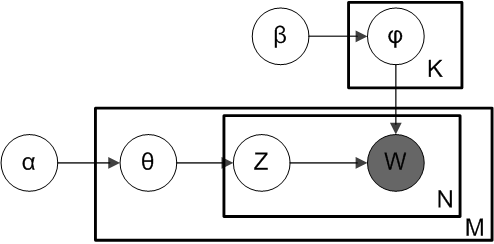
\includegraphics[scale=0.48]{figs/Smoothed_LDA}
\caption{Plate Diagram of LDA.}
\end{figure}

\begin{figure*}[ht]
	\centering
	\includegraphics[width=\textwidth, height=75mm]{figs/topwordsorig}
	\caption{Original barchart of the top 20 words and their counts.}
	\includegraphics[width=\textwidth, height=75mm]{figs/topwords}
	\caption{Barchart of the top 20 words and their counts after preprocessing.}
\end{figure*}


\begin{filecontents}{jobname.bib}
@incollection{zhao2011comparing,
	title={Comparing twitter and traditional media using topic models},
	author={Zhao, Wayne Xin and Jiang, Jing and Weng, Jianshu and He, Jing and Lim, Ee-Peng and Yan, Hongfei and Li, Xiaoming},
	booktitle={Advances in Information Retrieval},
	pages={338--349},
	year={2011},
	publisher={Springer}
}
@inproceedings{hong2010empirical,
	title={Empirical study of topic modeling in twitter},
	author={Hong, Liangjie and Davison, Brian D},
	booktitle={Proceedings of the first workshop on social media analytics},
	pages={80--88},
	year={2010},
	organization={ACM}
}
@inproceedings{cheng2010content,
	title={You Are Where You Tweet: A Content-Based Approach to Geo-locating Twitter Users},
	author={Z. Cheng, J. Caverlee, and K. Lee},
	booktitle={Proceeding of the 19th ACM Conference on Information and Knowledge Management (CIKM)},
	month={October},
	year={2010}
}
@article{blei2003latent,
	title={Latent dirichlet allocation},
	author={Blei, David M and Ng, Andrew Y and Jordan, Michael I},
	journal={the Journal of machine Learning research},
	volume={3},
	pages={993--1022},
	year={2003},
	publisher={JMLR. org}
}
\end{filecontents}

\nocite{*}

\bibliographystyle{abbrv}
\bibliography{jobname}

%\balancecolumns 

\end{document}